The HAT-P-37 system is present in 11 different sectors of TESS with a cadence of 120.0 s. Previously timing data from only one sector (59) has been published \citep{wangLongtermVariationsOrbital2024}. Upon investigation, 8 out of the 10 unpublished sector lightcurves produced by the TESS-SPOC pipeline in the lightkurve package show significant contamination of the HAT-P-37 flux. Using the MAST database \COM{add citation?}, we were able to determine that the main source of this contamination was a nearby variable star, ZTFJ185715.34+511631.4, which is a W Ursae Majoris (EW)-type Eclipsing binary, as characterized by \cite{chenZwickyTransientFacility2020}. For simplicity, we will refer to this star as "EB" from here on. 

Using the orbital period from \cite{chenZwickyTransientFacility2020} and the tools in the lightkurve package, we have been able to separate the transit light curves for HAT-P-37 b from the variability of the EB. Figure \ref{fig:EB_folded} depicts all 11 sector's PDCSAP flux phase folded to the parameters of the EB as published previously. This figure shows that the amount of contamination varies from sector to sector, leading to a sector specific approach being necessary to remove the contamination and fit the transit light curves of HAT-P-37 b. Table \ref{tab:crowding_params} lists the flux fraction and crowding metric of each TESS sector as defined in \cite{stumpeKeplerPresearchData2012}. This data also shows that Sectors 59, 74, and 75 have the lowest flux fraction which means they are the least contaminated further supporting that those data do not need to be treated in a special manor. Because of this the mid-times reported for Sectors 74 and 75 were determined by the analysis as described in \citep{adamsDoomedWorlds2024}, and the mid-times reported for Sector 59 are as reported in \citep{wangLongtermVariationsOrbital2024}. 

\begin{figure}
    \centering
    \includegraphics[width=0.6\linewidth]{figures/all_sectors_folded_EB_period.png}
    \caption{TESS sectors phase folded on the period of the EB. Each sector is affected by a different amount of contamination and as such each sector will need to be detrended separately.}
    \label{fig:EB_folded}
\end{figure}

\begin{table}[]
    \centering
\begin{tabular}{|c|c|c|}
    \hline
    Sector & flux fraction & crowding metric \\
    \hline
     26 & 76.932538 & 0.50555998 \\
     40 & 65.789335 & 0.67453253 \\
     41 & 66.98885 & 0.66584015 \\
     53 & 60.779458 & 0.6333406 \\
     54 & 64.582843 & 0.6583783 \\
     55 & 74.128646 & 0.52300292 \\
     59 & 58.385509 & 0.74245846 \\
     74 & 59.20288 & 0.69401199 \\
     75 & 59.999548 & 0.72226816 \\
     80 & 65.208763 & 0.62719065 \\
     82 & 66.821003 & 0.63547468 \\
     \hline
\end{tabular}
    \caption{Values of the Flux Fraction and Crowding Metric as defined in \cite{stumpeKeplerPresearchData2012} for all sectors of HAT-P-37 b}
    \label{tab:crowding_params}
\end{table}

\begin{figure}
    \centering
    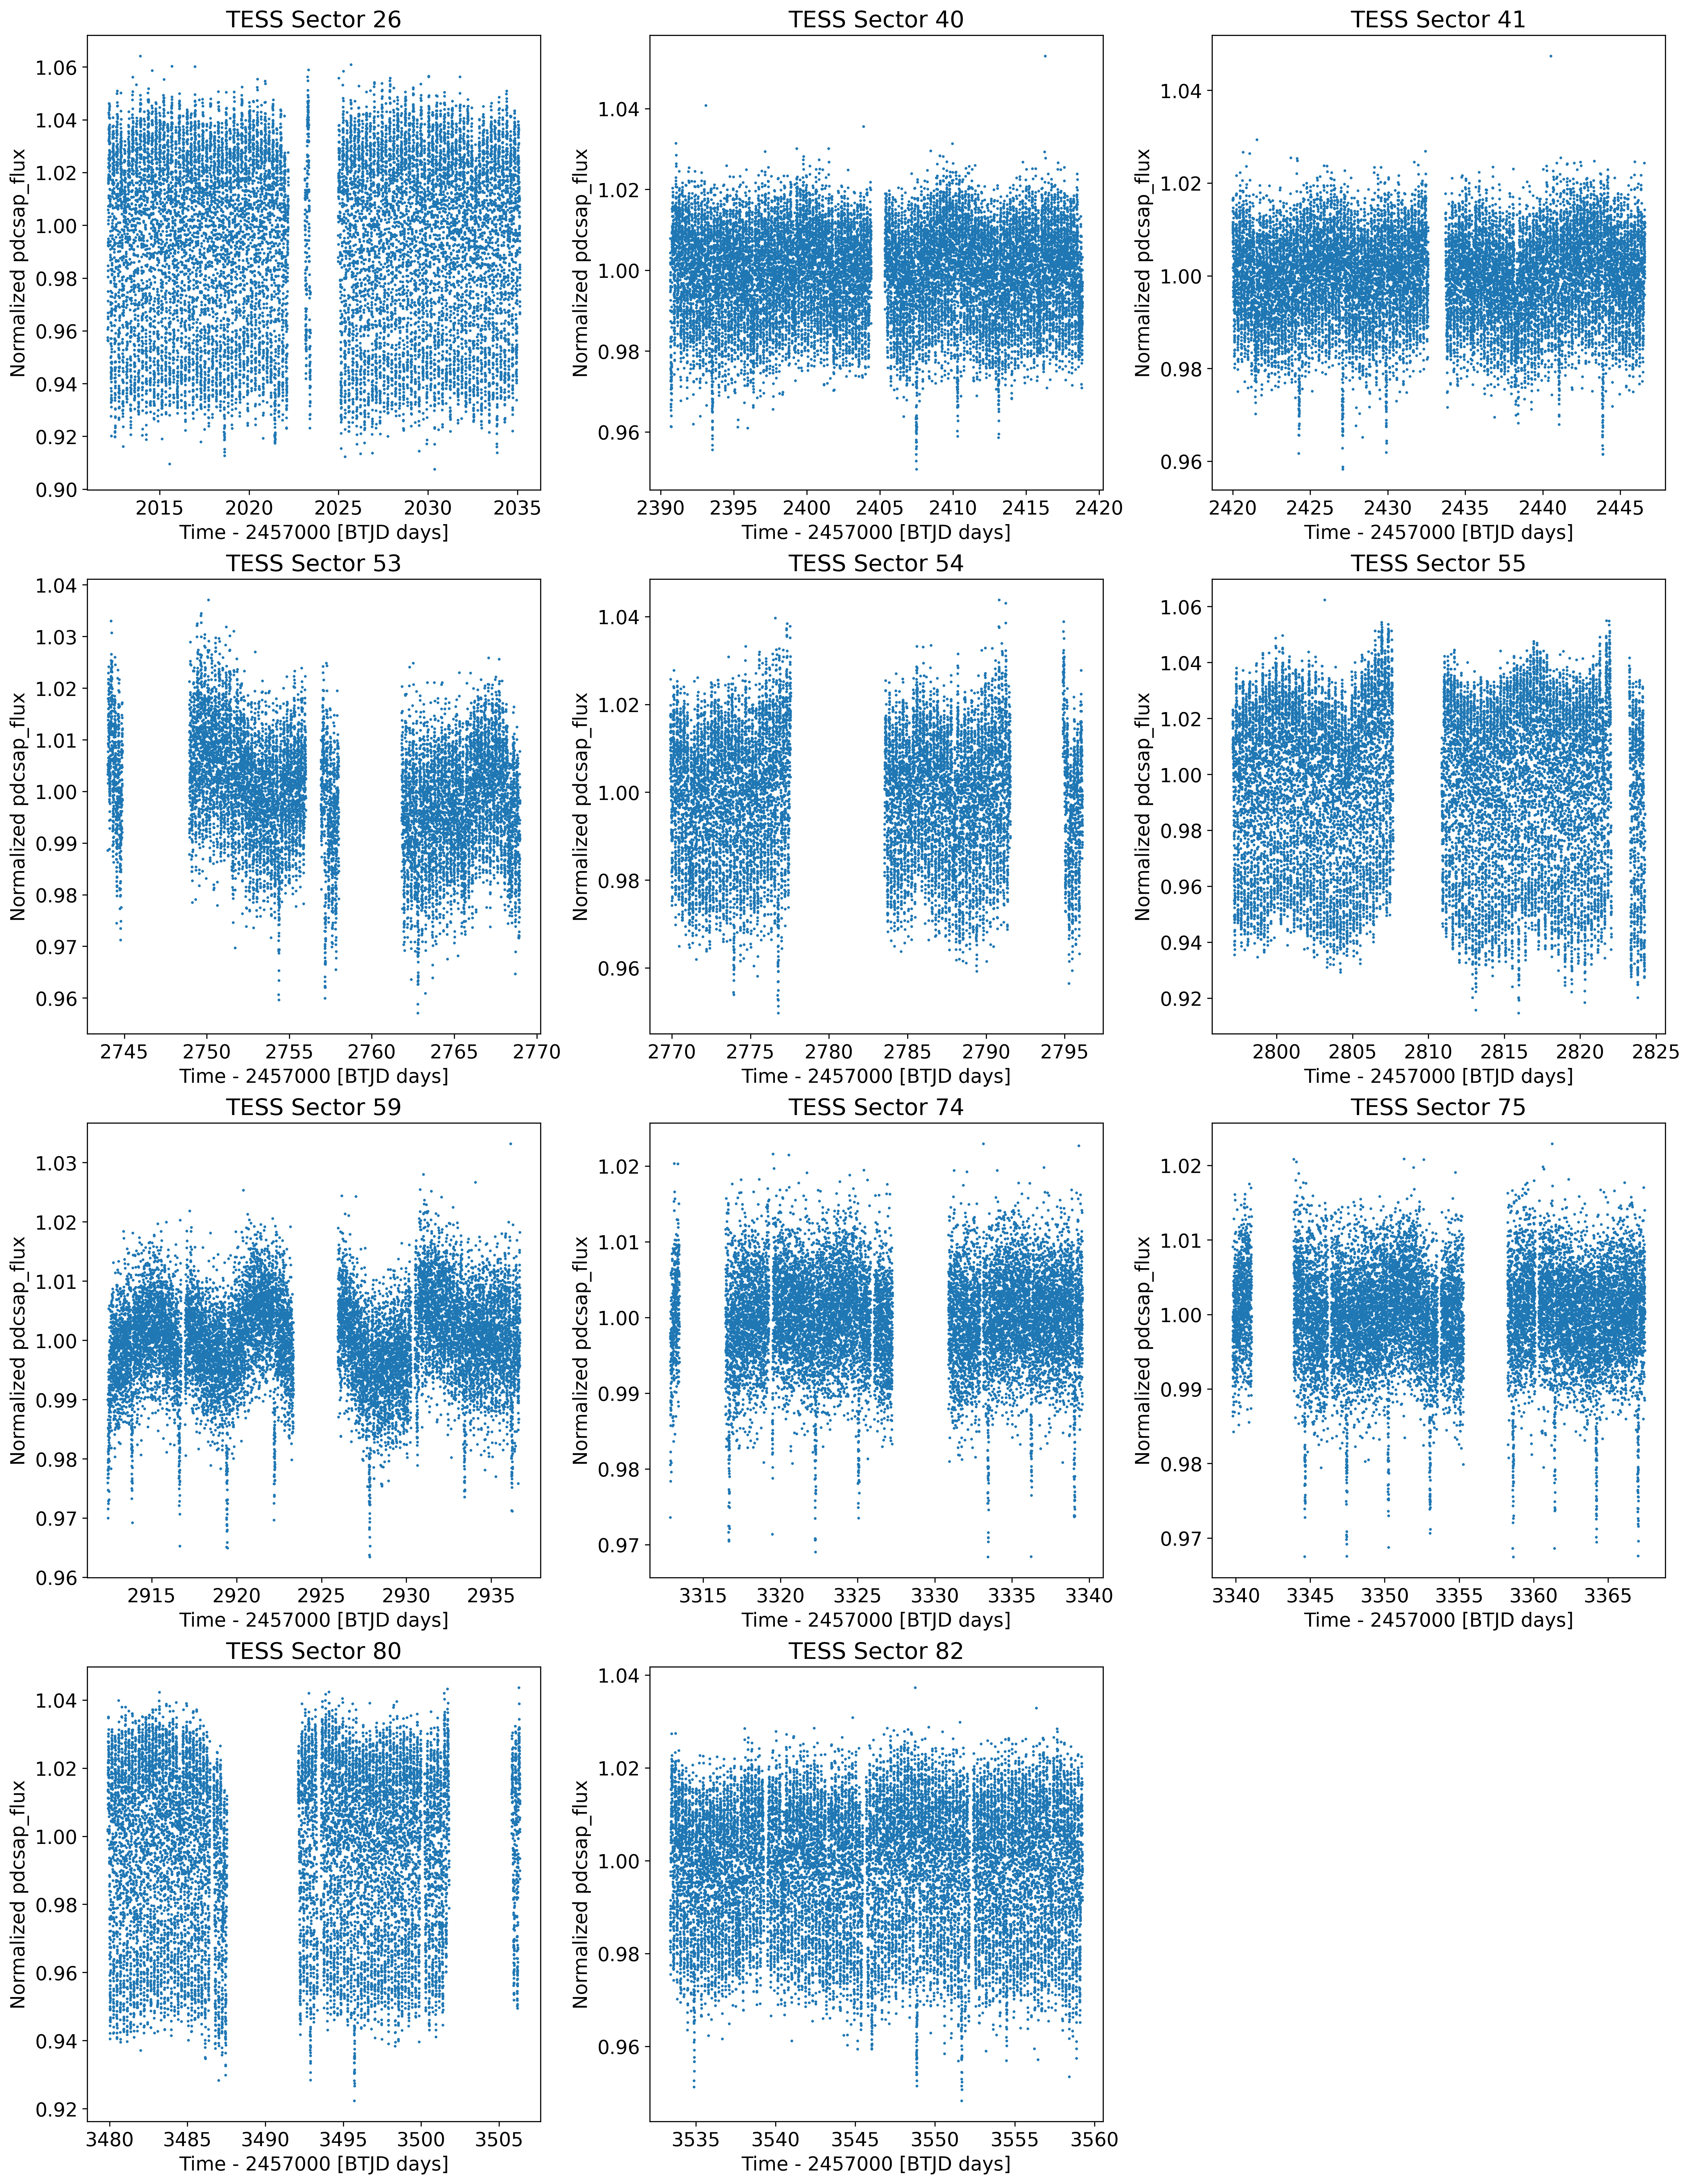
\includegraphics[width=\linewidth, height=0.8\textheight, keepaspectratio]{code/figures/allSectors_sigma5_PDCSAPflux_lc.png}
    \caption{PDCSAP flux for each sector of Tess data}
    \label{fig:enter-label}
\end{figure}



\begin{figure}
    \centering
    \includegraphics[width=\linewidth]{figures/wellbehaved_sectors_LS_periodogram.png}
    \caption{Lomb-Scargle Periodogram of the TESS sectors used in this study. Each sector returns a period at maximum power approximately one-half of the expected period of that of the EB.}
    \label{fig:LS}
\end{figure}

For these contaminated sectors, we apply the following detrending analysis. First, 